\chapter{Research Description}
\label{sec:researchdesc} 

\section{Introduction}
\label{sec:introduction}

\section{Background of the Study}
\label{sec:backgroundstudy}

% What is NA Quantification and its applications ? %
Quantification of Nucleic acids (NA) is a developing research field in molecular biology for the detection and quantification expression levels of genes \cite{Huggett2015}. These NA molecules are found in deoxyribonucleic acid (DNA) and ribonucleic acid (RNA), which carries genetic information and is used as biomarkers for the detection of diseases. Additionally, along with the rise of bioinformatics tools, NA quantification methods are also utilized in rare mutation detection, copy number variation detection, single-cell gene and microRNA expression analysis, and next-generation sequencing \cite{Quan2018}. Outside the scope of molecular biology, its application has also found its way in forensic research \cite{Whale2013}, medical diagnosis, environmental monitoring, and food safety analysis \cite{Cao2017}.


% How to Quantify NA Quantification with (dPRC) ? %
To be able to determine the concentration of target NAs, NA detection is naturally a pre-requisite. There are, however, NAs of interests that have very low concentrations to the point that it becomes undetectable in existing detection technologies. This problem is solved by amplifying the NA sequences using Polymerase Chain Reaction (PCR), a widely-used method for NA amplification since its invention in the 1980s \cite{Cao2017}. PCR can multiply specific NA sequences in DNA or RNA from low concentrations to millions of copies. This method exposes the NA sequences mixed with chemical components in a series of 20 to 40 temperature cycles. In each cycle, PCR doubles the NA molecule; theoretically producing \(2^n\) molecules after \(n\) cycles \cite{Quan2018}.

After PCR amplification, absolute NA quantification is achieved using digital Polymerase Chain Reaction (dPCR) technique. This equally divides the NA samples into thousands of partitions; each of these partitions is evaluated as either off or on, or in this context, labeled as positive or negative, hence the term "digital" \cite{Cao2017}.

The dPCR workflow, as illustrated in \figref{fig:dpcrWorkflow}, is usually a sequential procedure of extracting the sample from an organism, concocting the sample with several chemical components into a reaction mix, distributing the reaction mix to equal partitions, amplifying and detecting the target molecules using PCR, and the concentration is then finally estimated using a Poisson correction factor. In \cite{Jacobs2014}, it was emphasized that every step of the dPCR workflow inevitably allows for the introduction of different sources of variation. These variance components within the dPCR workflow is shown in \figref{fig:workflowVariation}. 

\begin{figure}[h]
    \centering
    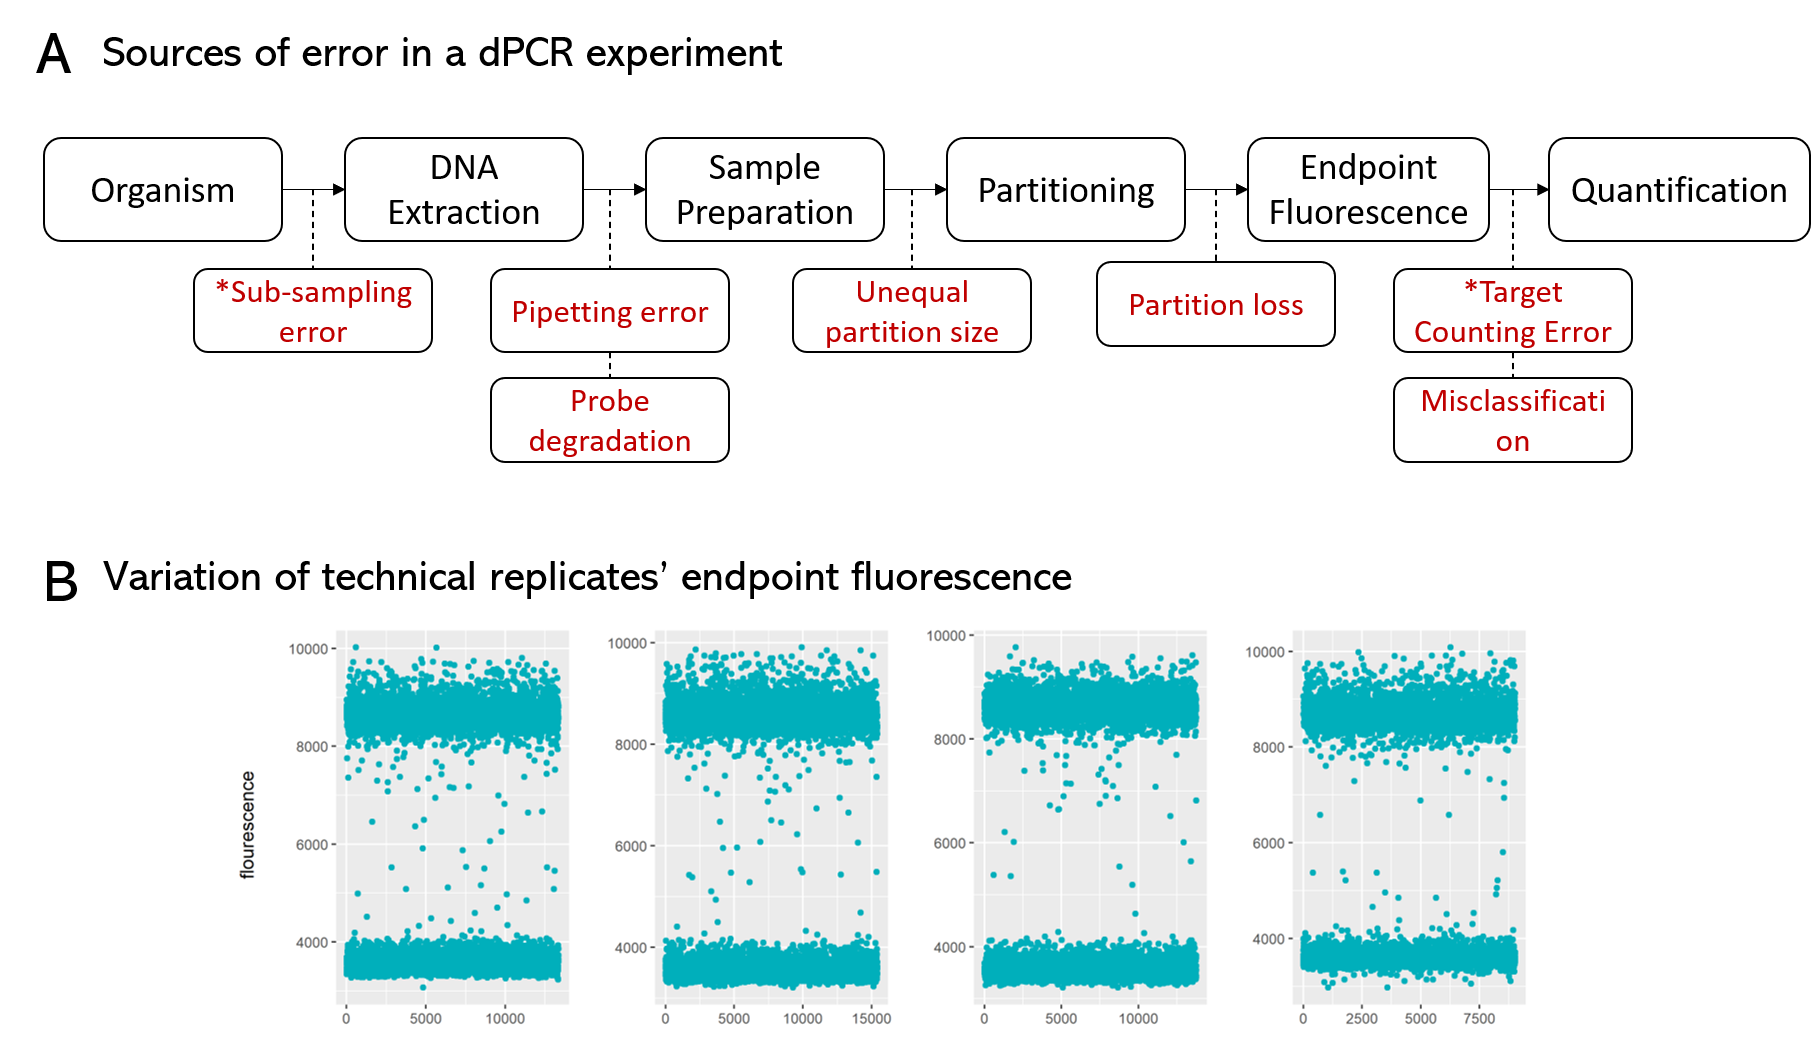
\includegraphics[max size={\textwidth}{\textheight}]{dpcrWorkflow.png}
    \caption{The dPCR workflow}
        \label{fig:dpcrWorkflow}
\end{figure}

\begin{figure}[h]
    \centering
    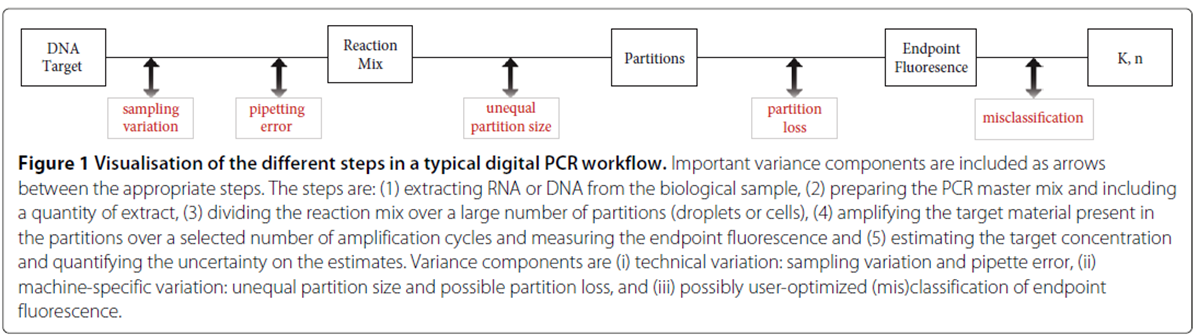
\includegraphics[max size={\textwidth}{\textheight}]{workflowVariation.png}
    \caption{Potential variation components between steps of the dPCR workflow}
        \label{fig:workflowVariation}
\end{figure}

Sampling variation stems from the fact that only a small sample of the organism is extracted; and although there is an expected number of target molecules per liters of a sample, drawing equally sized samples will result in different target molecules that are more or less near the average. \shortciteA{Tzonev} demonstrates the number of target molecules that can be drawn from extraction is distributed as Poisson. Besides the sampling error, samples may also exhibit imperfections, and thus have inhibited amplification. 

Preparing the reaction mix is a delicate process that strictly requires the accuracy of the pipetting volume; and yet, technical variation still occurs that results in pipetting errors. The next variation components are the possibility of the distributed partitions to be of unequal volumes and the loss of partitions due to physical interventions. Finally, upon PCR amplification, each droplet partition emits an endpoint fluorescence that would be used to classify the partition as positive or negative. However, some partitions are difficult to classify due to inhibition, delayed reactions, primer depletion, and other biological factors.

Each variance component accumulates to the bias and variance of the final estimated target molecule concentration, and thus, this gives rise to the importance of providing solutions that would increase precision in every step. To increase the sensitivity and specificity of the estimate, the misclassification of droplet partition should be minimized as much as possible. A high presence of false-negative droplets reduces sensitivity, while specificity is lowered for high false-positive count. Due to the variance contributed by misclassification, \shortciteA{Tzonev} recommends reporting the rates of false positives (FPR) and false negatives (FPN) per partition. More importance is given to either of the two depending on the kind of test being performed. If the total negative partition is expected to be large, then there is more chance that a true negative partition may turn into a false positive reading; which in this case, FPR may be of more interest than FNR. 

The primary problem in misclassification lies in 'rain' droplets; these are partitions that emits an intermediate fluorescence signal that is difficult to classify as positive or negative. Figures \ref{fig:plate1cru} and \ref{fig:plate1tc1507} demonstrates two different DNA targets with the former showing a visually clearer distinction of the positive and negative population than the latter, of which is possessing multiple rain droplets. The data used in these figures are sourced from the publicly available dataset from the study of \shortciteA{Lievens2016}. 

\begin{figure}[h]
    \centering
    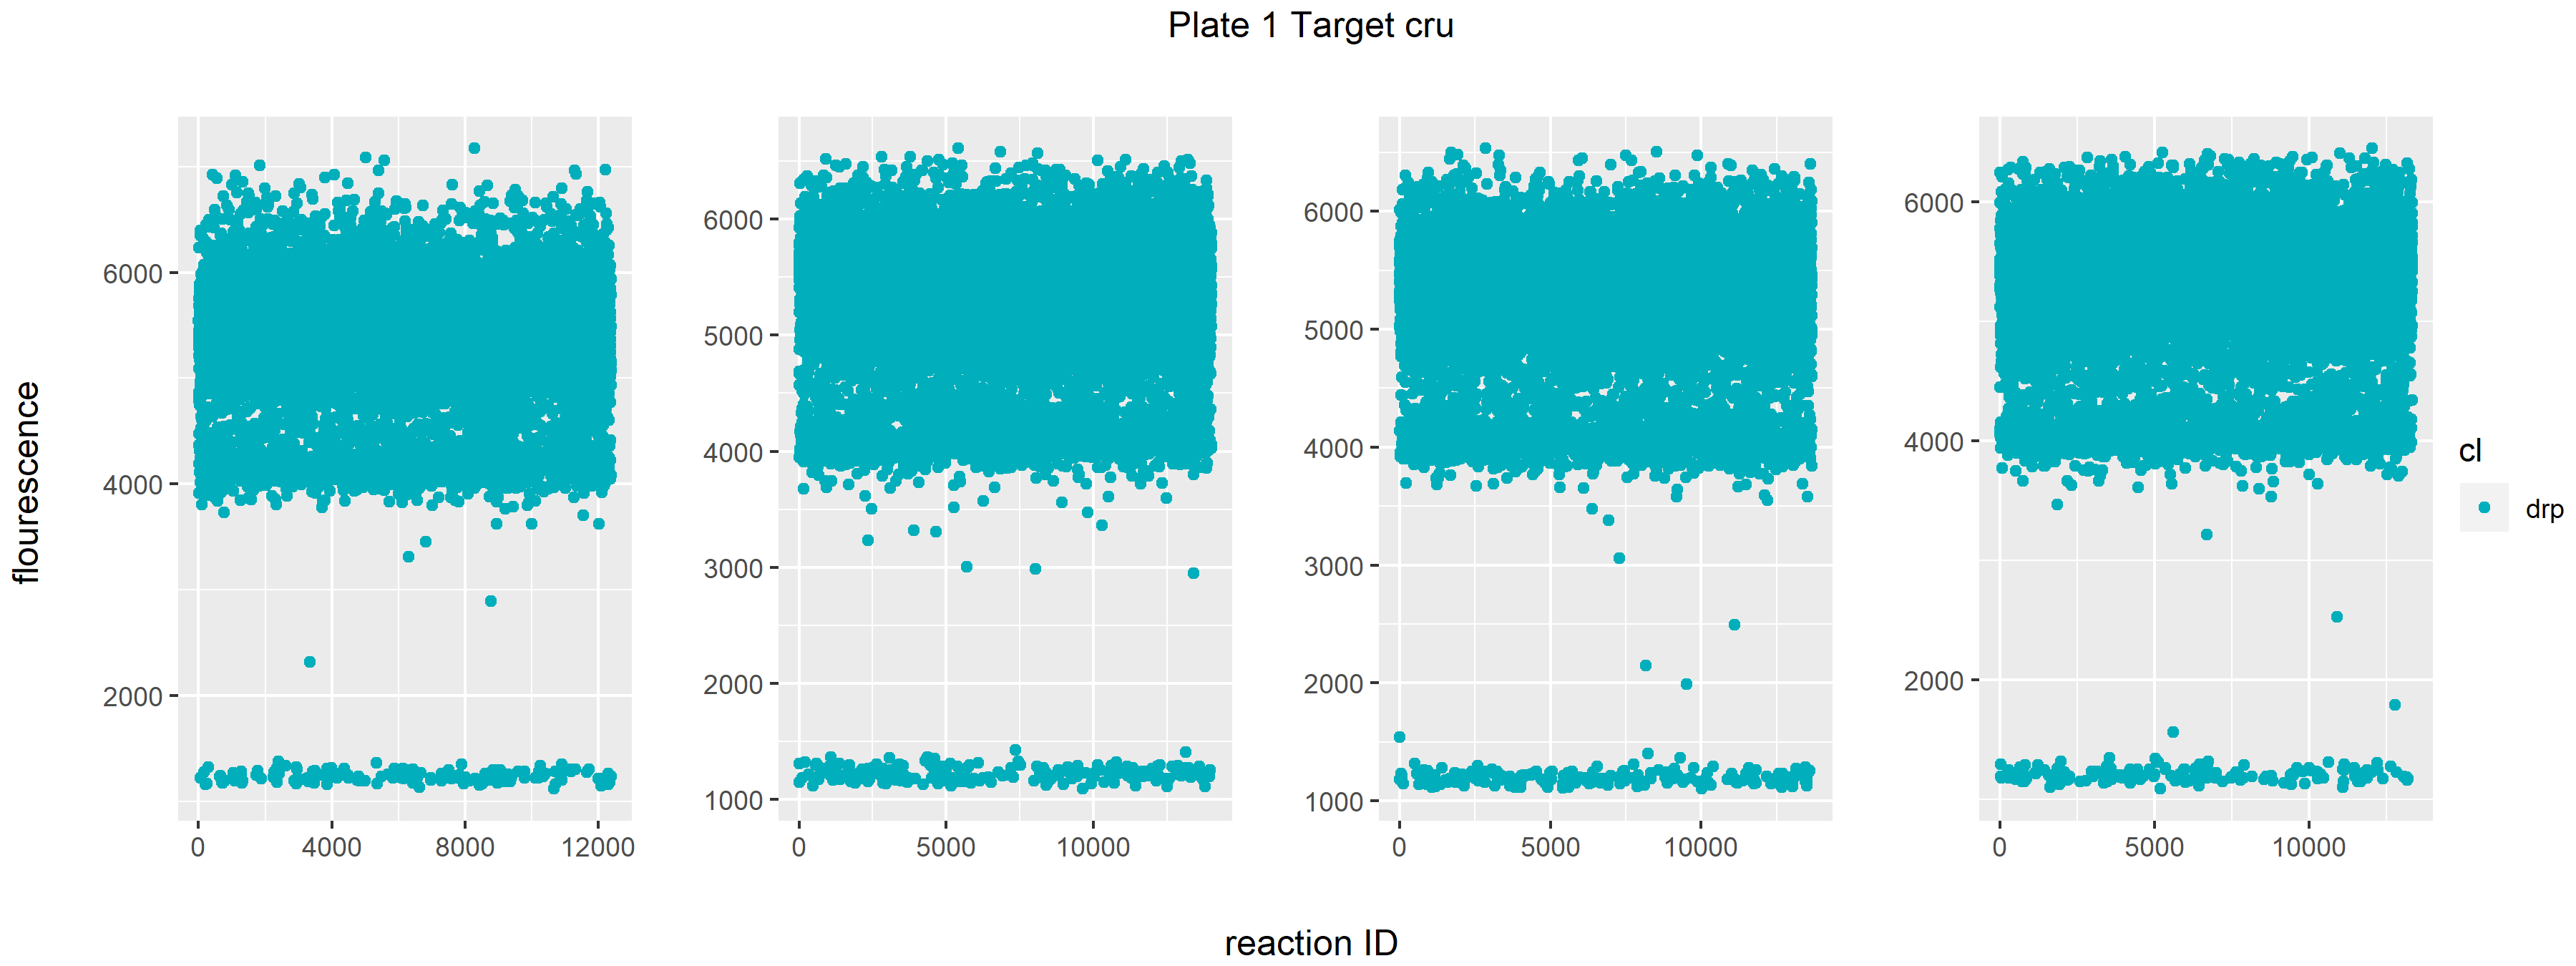
\includegraphics[max size={\textwidth}{\textheight}]{Plate 1 Target cru.png}
    \caption{Fluorescence readings of 4 repititions of DNA target cru}
        \label{fig:plate1cru}
\end{figure}

\begin{figure}[h]
    \centering
    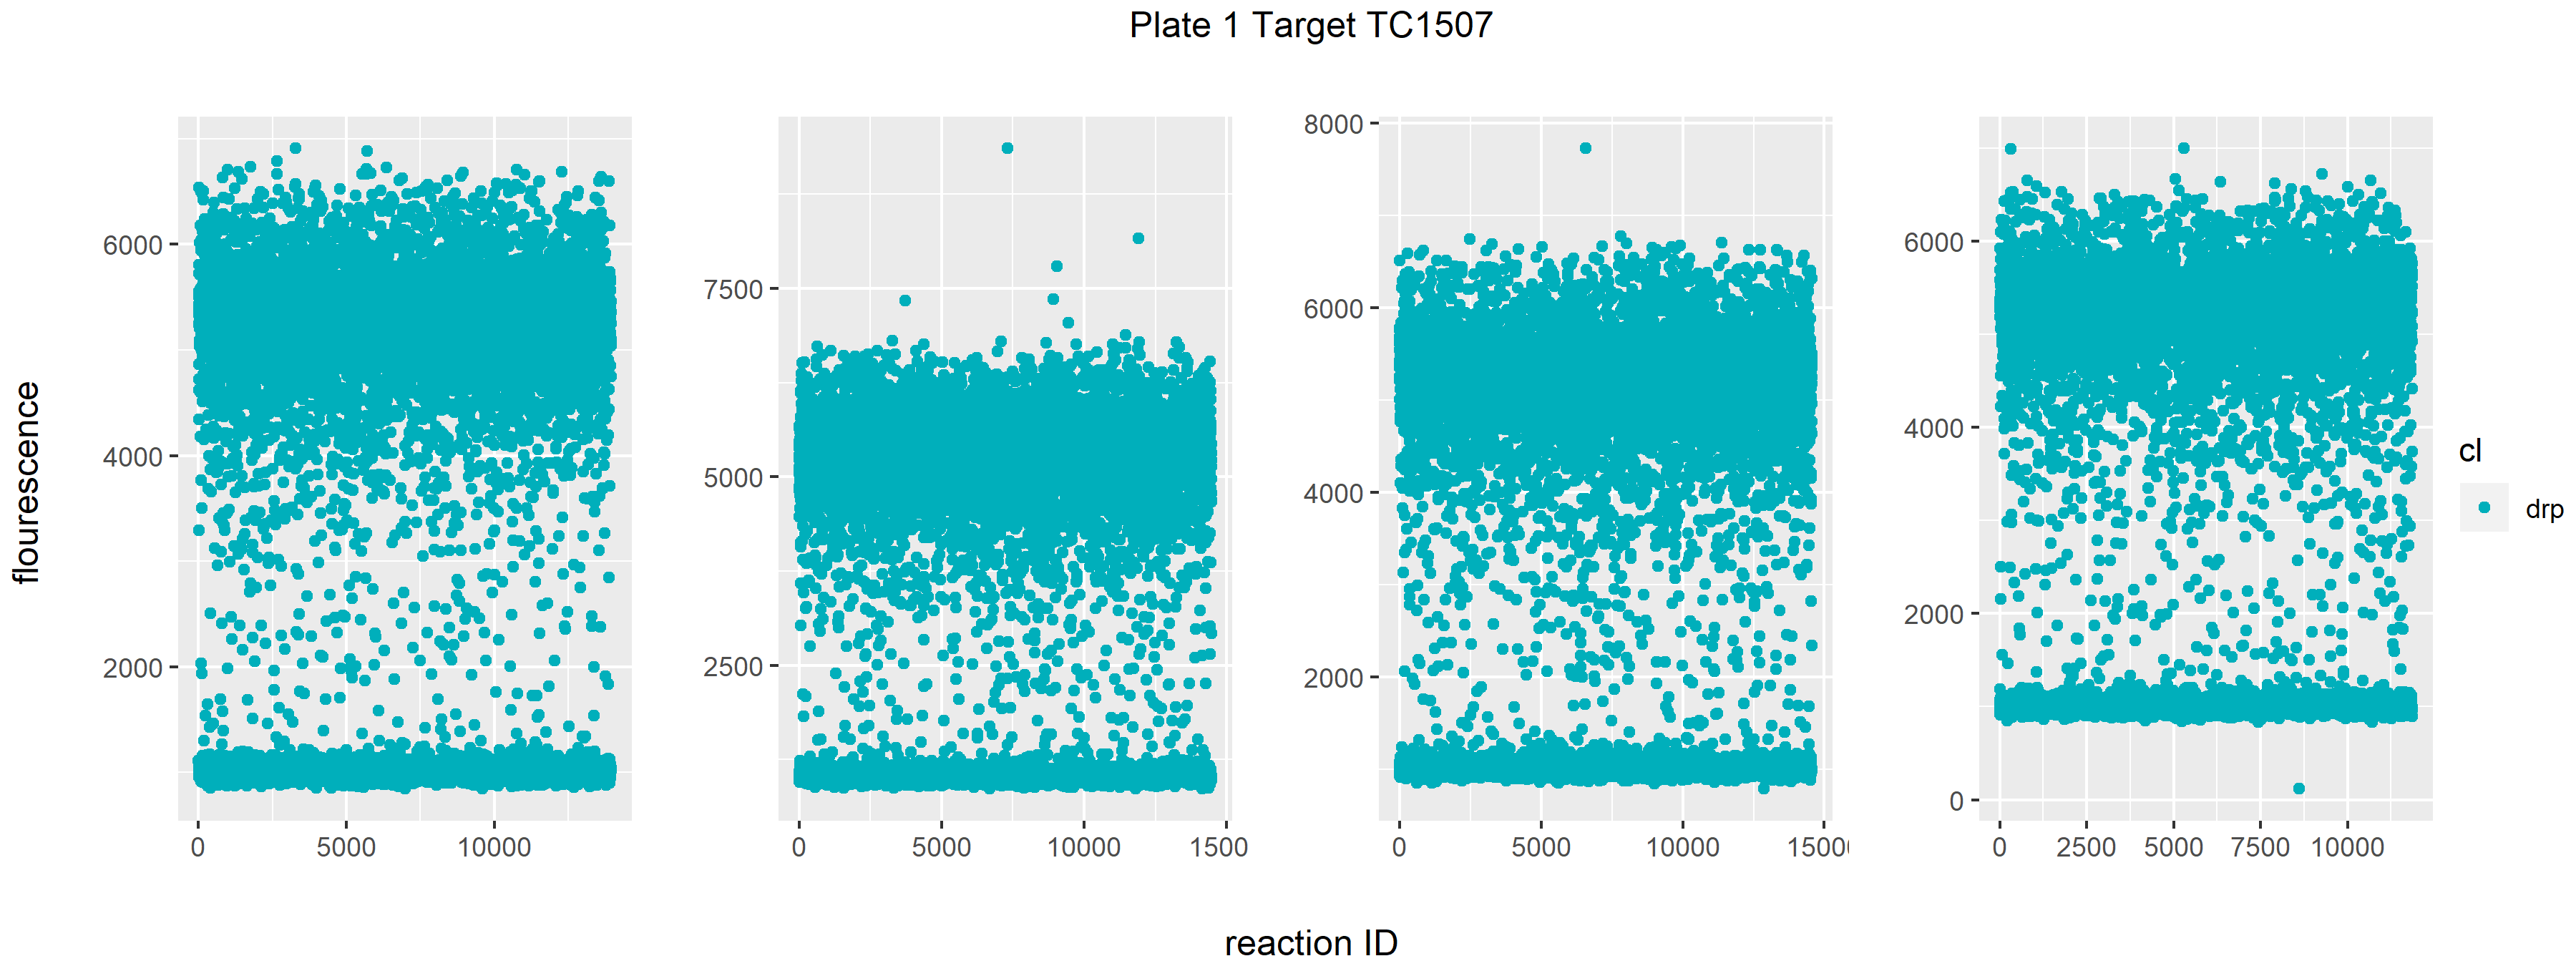
\includegraphics[max size={\textwidth}{\textheight}]{Plate 1 Target TC1507.png}
    \caption{Fluorescence readings of 4 repititions of DNA target TC1507}
        \label{fig:plate1tc1507}
\end{figure}

The estimate for DNA target concentration highly depends on the positive and negative classifications. For experiments with low copy DNA targets, the focus is on maximizing the sensitivity of the test for these very small number of positive droplets. Low sensitivity translates to failure in detecting lower concentrations. 

For assays with large differences in the distance between the two fluorescence groups (positive and negative droplets), most quantification tools estimate the target concentrations with high sensitivity. As exhibited in an optimized assay experiment of E. amylovora \cite{Dreo2014}, slight differences of thresholds calculated from different tools had little effect on the final estimated concentration. However, for R. solanacearum, which is observed to manifest false-positive signals in qPCR experiments, produces unsatisfactory analytical sensitivity of the concentration estimates. 


% \citeA{Jones2014} stresses the impact of false positives for DNA targets of low copy numbers. This is because the count of false positive droplets will highly influence the relative proportion of total positive droplets. %

The danger of false rates due to misclassification is expounded at the clinical level, where false rates lead to the misdiagnosis of patients \cite{Tzonev}. One such case is the prenatal screening test for Down Syndrome; this test is expected to mostly result in normal pregnancies. However, even for a small FPR, many pregnancies are still falsely reported as positive for Down Syndrome. False negatives also risk the overall health of the patient that truly possesses the genetic disorder.




\section{Statement of the Problem}
\label{sec:statementprob}

This thesis aims to classify dPCR droplet partitions into positive or negative by exploring Model-Based clustering with Expectation Maximization. The specific objectives of this study are to:
\begin{enumerate}
    \item Fit two-component finite mixture densities on the datasets with varying amounts of rain and increasing target DNA concentration;
    \item Classify partitions using the fitted models for each experiment and estimate DNA concentration using the standard formula;
    \item Evaluate and compare the precision and bias of the estimates amongst the existing classification methods. 
\end{enumerate}

\section{Significance of the Study}
\label{sec:significancestudy}
Quantification of target concentrations for pathogenic bacteria, gene expression of diseases, cancer diagnostic, and other health-related applications strongly demand estimators with high sensitivity and precision, as lives are put to risk for false-positives. A modern approach to DNA and RNA target quantification is through the dPCR method. In one of the steps of the dPCR workflow, the classification of droplet fluorescence still has areas of improvement. 

The most prominent problem in classification lies in experiments exhibiting a high frequency of rain, or intermediate fluorescence values. These are experiments that have not yet been optimized. As different DNA target samples exhibit distinct structures \cite{Lievens2016}, an optimized setup for one DNA target may not be applicable for other targets. Additionally, for samples with low concentration, the total count of detected positive droplets dramatically changes the final concentration estimate, due to the greater impact of false positives in the proportion of detected over the number of true positives. The following are some tools and methodologies proposed for droplet classification: Quantasoft propriety software, definetherain \cite{Jones2014}, manual global threshold \cite{Dreo2014}, cloudy \cite{Lievens2016}, and Umbrella \cite{Jacobs2017}. Most of the aforementioned droplet classifying tools rely strongly on how representative reference samples are. According to \citeA{Dreo2014}, such approaches are sensitive to significant shifts in amplitude for previously unobserved factors, such as cross-reactions or the influence of inhibitors.

In an attempt to prevent the problem of representation, this study will explore the feasibility of estimating target concentrations without a reference sample. Similar to Umbrella, this study also aims to use model-based clustering for the droplet classification but with relaxing the assumptions using the Expectation-Maximization algorithm. The significance of the study will be useful in quantifying concentrations in targets that have not yet been optimized for dPCR experiments and also for quantifying targets of low concentrations. 

\section{Scope and Limitations}
\label{sec:significance}
This study solely relied on publicly available fluorescence datasets from published research papers. Only two were found and will be used for statistical analysis, namely from \shortciteA{Lievens2016} and \shortciteA{Jones2014}. The former dataset contains twelve DNA targets from food and feed samples ran on nine different settings by controlling for experimental factors; the latter dataset is a serial dilution of the Albumin DNA ranging from \(10^0\) to \(10^5\) copies. 

The droplet classification method in this study uses model-based clustering, or the use of finite mixture models to perform clustering. However, the identification of the distribution of the mixture densities will be dependent on the observed available dataset. As a consequence of the limited dataset, the paper's methodology described here needs more study for other experimental setting and nucleic acid targets.

Lastly, statistical results presented may lack biological explanations which could be useful for explaining the variances of the droplet fluorescence. Such information may be utilized to further improve the estimation process.